%------------------------------------------------------------------------------
%Description       : DDMoRe WP7.2.1 First Technical Specification for the Model
%                                   Repository Infrastructure - Proposed Design 
%Author            : Mihai Glonț <mglont@ebi.ac.uk>
%Organization      : EMBL-EBI
%                    Wellcome Trust Genome Campus
%                    Hinxton
%                    Cambridge
%                    United Kingdom
%------------------------------------------------------------------------------
\section{Direct interaction with the \ddmore Model Repository}
\label{directInteraction}
Having defined the context and the needs of the \ddmore Model Repository, we now proceed to describe the capabilities and behaviour of the envisaged solution. We present a high-level view of the features that will be available. A comprehensive list of scenarios 
%along with low-fidelity designs 
illustrate how each of the stakeholders from Section~\ref{users} interacts with the system. Each such interaction is called a \gls{usecase}, while the user performing it is known as an \gls{actor}. The use cases listed in Figure~\ref{fig:useCases} only consider the main actors that are involved, hence Administrators are not mentioned in any model-related use cases, in spite of the fact that they do have the authority required to perform any action.

\begin{figure}[htb]
\centering
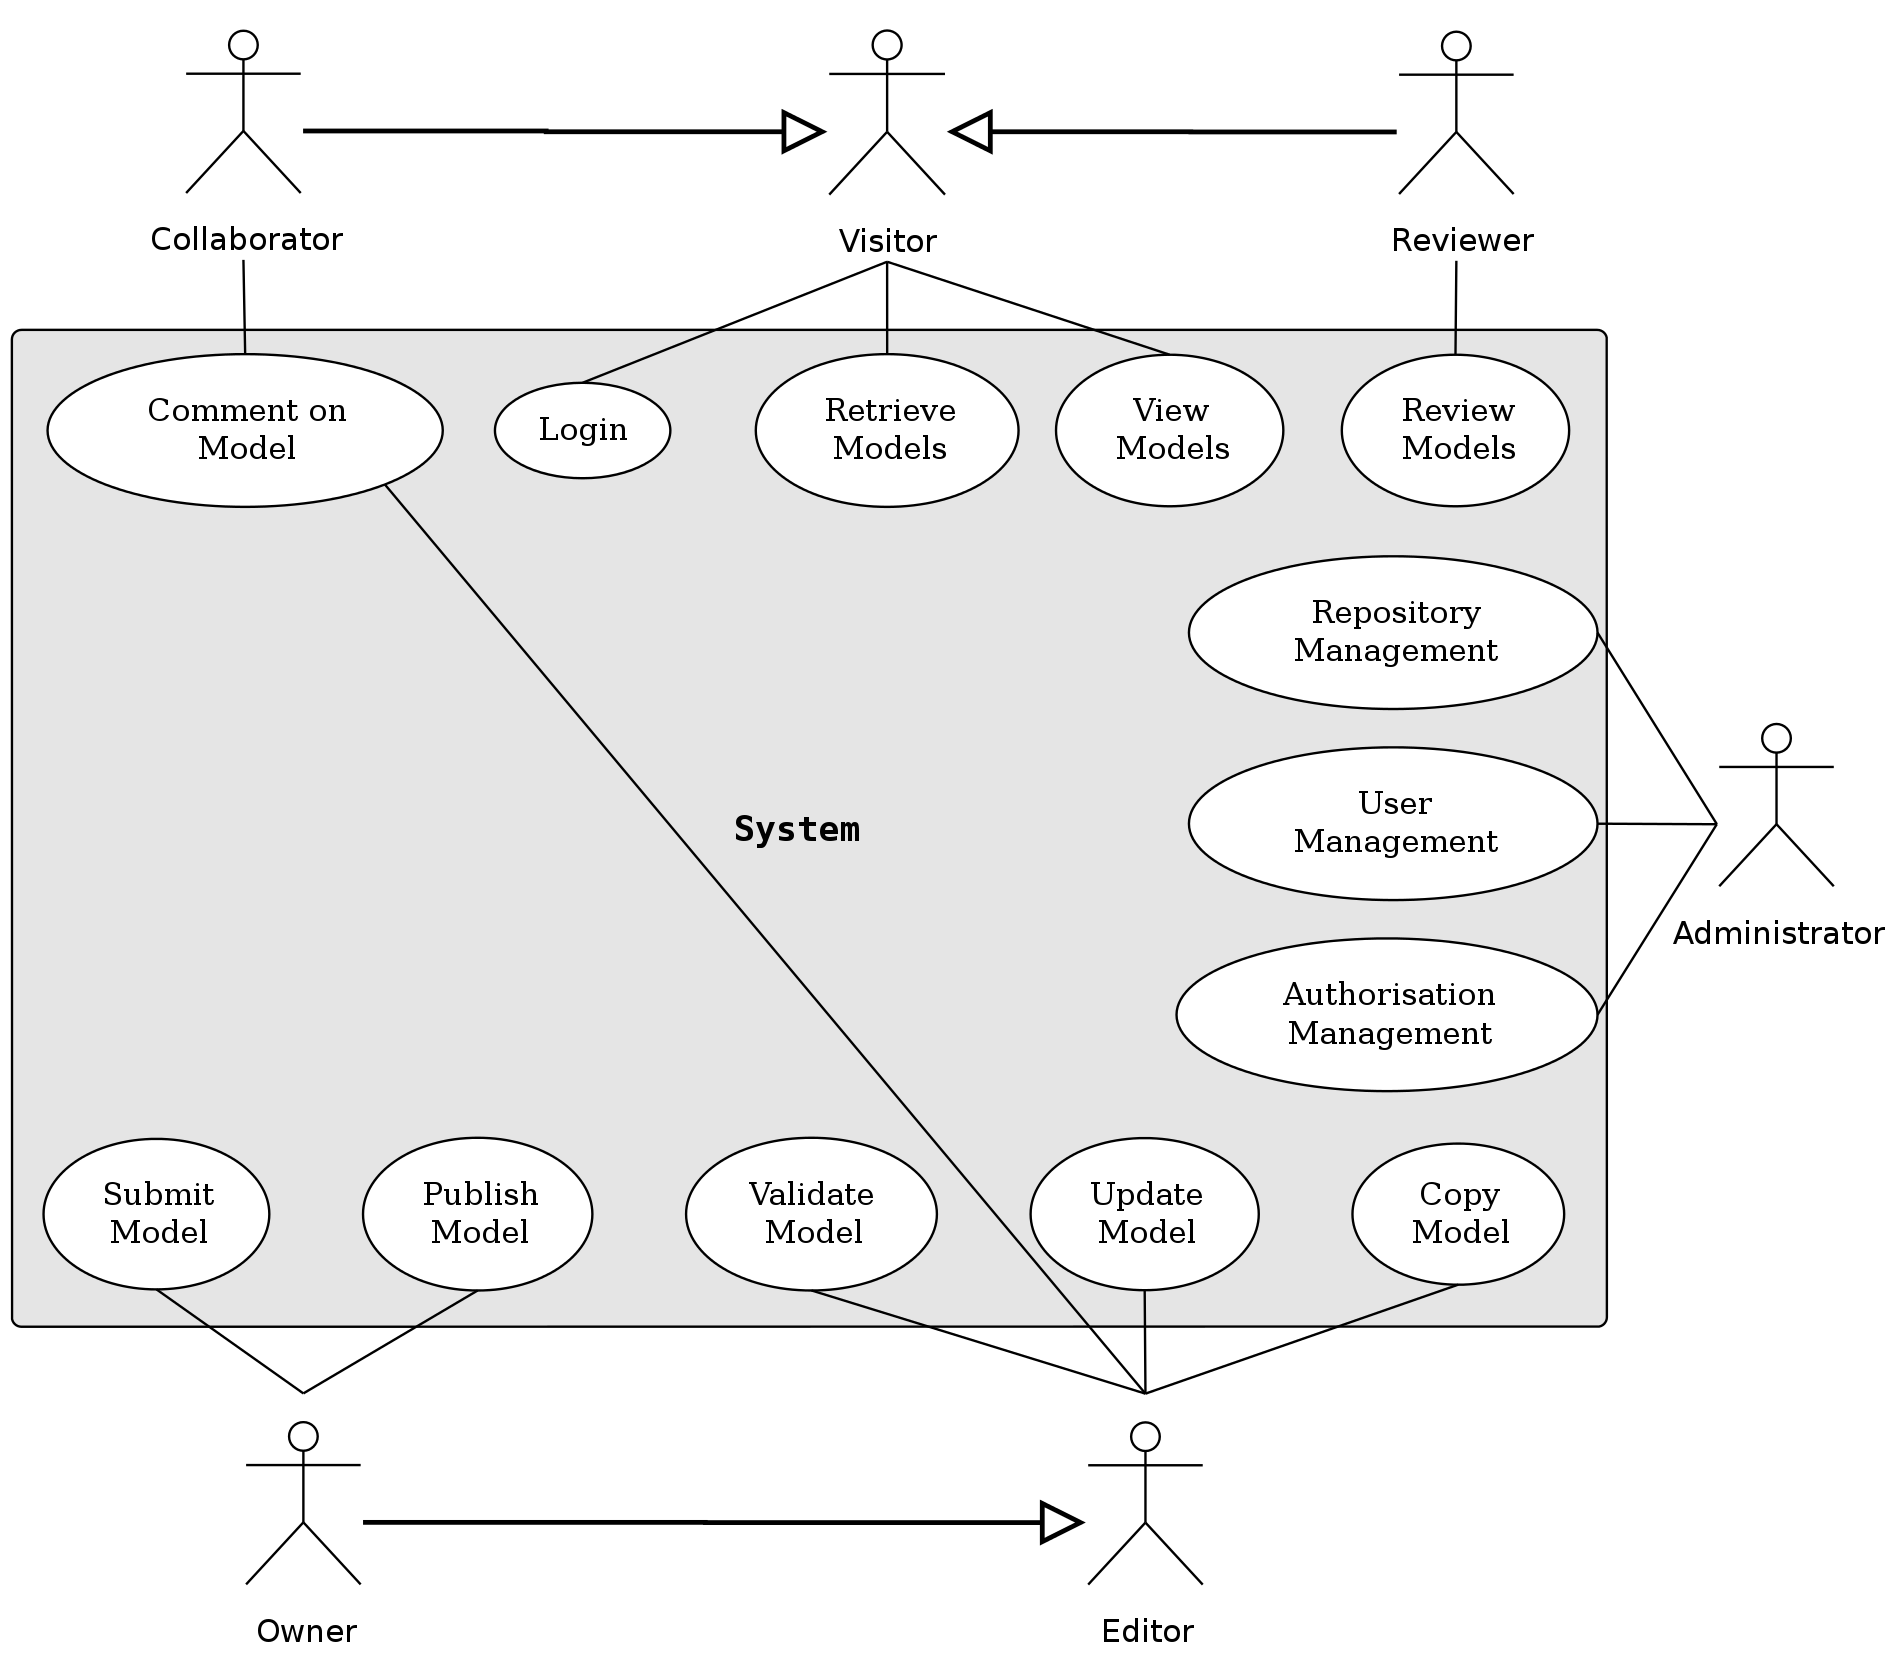
\includegraphics{img/UseCases}
\caption{Diagrammatic representation of the system's scope.}
\label{fig:useCases}
\end{figure}

\subsection{Initial considerations}
\subsubsection{User profiles}
\label{userProfiles}
The scenarios listed below are illustrated from the perspective of the following users:
\begin{description}
    \item[Joe] -- scientist interested in preclinical models of prostate cancer.
    \item[Sam] -- an Administrator of BestModels, a private instance of the \ddmore Model Repository used internally at BestMeds PLC, a large pharmaceutical company.
    \item[Hannah] -- a highly experienced PKPD modeller working at BestMeds PLC that has contributed to the development of many models which are deposited in BestModels.
    \item[Julia, Dominic, and Sue] -- young, but very promising modellers that have recently joined BestMeds PLC.
\end{description}

\subsubsection{MML Structure}
At the time of this writing, the specification of MML is under development. Given that features such as model submission, template creation, publication, search, or model display are dependent on the MML structure, there is a limited amount of information we can include about them at this stage. The discussion of these sections will be expanded once MML becomes publicly available.

\subsection{Model development}

\subsubsection{Submitting a model}

\idea{for public instance, this is the same as publishing. no authentication will be required. \textbf{ToDo: Write story about Joe that is studying the role of a particular type of flavonoid called Quercitin in inhibiting carcinogenesis.}}

\idea{
from homepage, click on \textsc{Submit a new model}; then the process depends very much on the structure of the MML, and the kind of model that you want to submit. however, we should start by collecting information about its creators. Then, we should validate the model and report any issues back to the submitter as grounds for rejecting the model. Once the model is deemed fit, we should extract any cross-references so that we can enhance the understanding of the model's context. Then, we store it and assign it a perennial identifier. we should also display a confirmation page right before we start processing the new model so that the submitter is offered a chance to correct incorrect details.
}

\idea{
for a private instance: User Login $\Rightarrow$ Display user homepage containing a list of models which (s)he has developed  $\Rightarrow$ User selects model  $\Rightarrow$ user chooses \textsc{Submit new version} from the list of actions that are available to them (action only appears when the user has write-access rights) $\Rightarrow$  pre-populate fields with information about the model $\Rightarrow$ user uploads the new version of the model $\Rightarrow$ display the list of collaborators that will have access to this revision based on the previous version $\Rightarrow$ user confirms access rights for this version $\Rightarrow$ display a summary of the model version that is about to be submitted $\Rightarrow$ user clicks \textsc{Finish} $\Rightarrow$ the new model version is processed.
}


\begin{techNote}
A Strategy pattern should be used, whereby each kind of model that is handled by that instance of the Repository corresponds to a class in charge of the submission algorithm; there needs to be a \texttt{SubmissionStrategy} interface containing a \texttt{submit} method. The Repository will have a plugin dedicated to each kind of model it supports. These plugins will implement the \texttt{SubmissionStrategy}. In addition, a \texttt{SubmissionManager} maintains a reference to a \texttt{SubmissionStrategy} object and is in charge of forwarding the submission responsibility to the correct plugin.
\end{techNote}

\subsubsection{Model Templates}
\emph{depends on the structure of the MML}

\subsubsection{Deleting models}
\idea{the revision owner (not the model owner) can delete a version, and then the Repository asks if there is a replacement version. The user has to be able to give a link to it, if it exists. Also, the user must be able to specify replacements for his(her) deleted versions at a later stage, so we need the concept of a Bin or Archive. As far as other users are concerned, when they access this model they should still see its contents, but there should be a clearly-visible message that stands out and informs them that this version is obsolete.
}

\subsubsection{Subscribing to model changes}

\begin{techNote}
we need a messaging system for this -- there is no efficient/scalable alternative. we store three kinds of notifications: 
\begin{itemize}
\item model-related -- new models, updates to the access rights of existing models
\item revision-related -- new revisions, deleted revisions, updated permissions, published revisions
\item comment-related -- new comments on existing revisions.
\end{itemize}
\textbf{Note: reviews are outside the scope of the notification system.}

Each \texttt{Model}, \texttt{Revision} and \texttt{Comment} therefore need to extend \href{http://docs.oracle.com/javase/6/docs/api/java/util/Observable.html}{\texttt{java.util.Observable}}. A \texttt{NotificationObserver} implementing the \href{http://docs.oracle.com/javase/6/docs/api/java/util/Observer.html}{\texttt{java.util.Observer}} interface will aggregate every change to every model, version, or comment. This object will be a \emph{Topic Publisher} in \emph{ActiveMQ} parlance -- a producer of messages. We will dedicate a \emph{Virtual Topic} to every user that expects notifications. At the other end, there will be a \emph{Consumer} in charge of forwarding the updates to the user. 
%We will have one queue per user that has subscribed to notifications about model updates. \textbf{translate into "english" that binding keys govern the routing process and that when a user clicks on "subscribe", we create a queue that captures all messages that start with modelID, regardless of what follows it.} The structure of the message needs to be agreed upon. We could use \texttt{source.action}
\end{techNote}


\subsubsection{Publishing a model}
% for public instance - the same thing as submitting
\idea{for private instances: user logs in $\Rightarrow$ user sees homepage containing his/her models $\Rightarrow$ user navigates to the display page for a model they own $\Rightarrow$ user views the section dedicated to model versions $\Rightarrow$ user clicks on the \textsc{Publish} button next to the version that needs to be published $\Rightarrow$ the version becomes available to all users. 
}

%for private instances, as a model owner, you go to "My Models", which is on the homepage of every authenticated modeller. 
%Click on the model you're interested in, which renders it in detail. You go to the \textsc{Revisions} section and select 
%the one(s) that you are interested in. Then you click publish. The system indexes the changes (\textbf{todo: decide when and how}) 
%and outputs a confirmation message if the action was performed successfully. 
%If it goes belly-up, then we could be in a lot of trouble, as data integrity could be compromised. 
%there will be no way of reverting the model from the VCS, not to mention the DB. The horror


\subsection{Model browsing, searching and retrieving}

\subsubsection{Browsing models}
\idea{user-friendly means of listing a potentially long list of models}

\subsubsection{Model display}

The user interface to show models will consist of the following blocks:
\begin{itemize}
\item model --
\item meta-data -- includes development history, creation/modification dates, authorship etcetera on the one hand, and clerical data on the other.
\item actions -- lists all actions that are available to the user, for instance parameter estimation, simulation, or download.
\end{itemize}

The display will depend on the model type and may vary from one instance of the Model Repository to another.

\subsubsection{Model search}
\idea{story about Joe, the Visitor of the public instance that surveys PK models of flavonoids and their influence on the human body. He performs a search using the term flavonoids.}

% As such, Joe, a Visitor of the DDMoRe Model Repository would have free access to the published models that are stored in that instance without needing to register or sign in. Joe would also be able to 

%\subsubsection{Advanced search criteria}

\begin{techNote}
we need to switch between searching the latest version of each model and every single accessible version. the easiest way to implement this would be to maintain two separate indexes, one for each type of search, but this will impact the time to generate them. 
\end{techNote}

\idea{include a scenario where private models are included in the search as well.}

\subsection{Model quality assurance}

\subsubsection{Model review}
\idea{as model owner: \textsc{Login} $\rightarrow$ navigate to the "My Models" section of their homepage $\rightarrow$ user selects the model for review $\rightarrow$ user clicks \textsc{Submit for review} button next to the version that should be reviewed $\rightarrow$ user selects reviewer and clicks \textsc{Finish} button $\rightarrow$ The model appears in the "Models under review" section of his homepage.\\%[1em]
for reviewer: \textsc{Login} $\rightarrow$ user navigates to the "Models I review" part of their homepage $\rightarrow$ reviewer clicks \textsc{Select Model} $\rightarrow$ the Repository displays the model $\Rightarrow$ reviewer selects the only action that is available: \textsc{Review} $\Rightarrow$ reviewer rates model quality using one of the scores below $\rightarrow$ user offers suggestions to the model developers in the form of textual comments $\rightarrow$ reviewer clicks \textsc{Submit review}.
\\%[1em]
Once the model enters the review process, it cannot be published until it is deemed fit by the reviewer.
}

\begin{techNote}
The quality of the model will be evaluated using one of the following grades, listed in descending order:
\begin{itemize}
\item Pass
\item Pass with minor changes -- minimum score required for a model version to be publishable
\item Major Changes required -- this will force the authors of the model to develop a revised version of it and will by default grant the reviewer access to the updated version. 
\item Reject
\end{itemize}
If the model gets published, reviews should not be displayed. 
\end{techNote}


\subsubsection{Model validation}
This will be performed automatically by the repository whenever a new model or version of a model is submitted. Users will also be able to do so by clicking on the \textsc{Validate} button next to each revision. A model will not be accepted in the Repository if it does not pass validation. 


\begin{techNote}
As simple as loading the model into the API developed by WP2.3, then calling its \texttt{validate} method; if validation failed, we rely on the API to provide the cause. We will then display those error messages back to the user.
\end{techNote}

\subsection{Repository management} 

\subsubsection{User registration}
\idea{the Administrator chooses whether new users can register themselves or not. The registration process will record \textbf{at least} the following user details:
\begin{itemize}
\item First Name
\item Last Name
\item username
\item password
\item email
\end{itemize}
}

\begin{techNote}
In order to prevent robots from registering, a CAPTCHA code should also be included. LDAP support will be provided, minimising the number of username and password combinations users need to remember. 
\end{techNote}


\subsubsection{Suspending accounts}
Due to irreconcilable differences with her manager, today is Hannah's last day at the office. Sam, therefore needs to revoke her access to the Repository from now onwards, so that she cannot steal company secrets. 

To achieve this, Sam logs in and navigates to the User Management section. Here he can see a list of all active and inactive users of the Repository displayed as a paginated table. From the list of actions that are displayed along each record, Sam selects \textsc{Disable account}, thus suspending Hannah's account. From now on, any attempt to log in using her credentials will result in an error message that will inform the user about the ban. The account will remain in the system for security purposes, hence Sam will be able to re-enable it, if need be.

\subsubsection{Creating user lists}
BestMeds PLC  wants to enhance the collaboration between the teams of modellers within the organisation. As such, Sam has been tasked to facilitate sharing a model with multiple people.

Consequently, he logs in to BestModels and navigates to the Team Management section. This contains a list of the names of all existing teams along with \textsc{Delete} and \textsc{View} buttons. Above and below this list there is a \textsc{Create team} button. By clicking on this button, Sam is taken to the page to create a new team. He types the name of the team --- \emph{PKPD-Modelling} --- and clicks \textsc{Confirm}. The system ensures that the team name only contains letters, digits, dashes (--) and underscores (\_) and then creates the new team. If Sam had named the team \emph{PKPD-Modelling-Rockstars!}, the Repository would have informed Sam about the problematic exclamation mark.

\subsubsection{Deleting user lists}
\idea{this action will cause users to lose access to certain models. discuss whether this is problematic.}

Sam logs in, goes to Team Management. Clicks on the \textsc{Delete} button next to the team he wishes to delete. He is advised that this will prevent members to access the models shared with the list and asked to confirm that he wishes to delete the list in question, being given the choice to \textsc{Confirm} or \textsc{Cancel}. Clicking on the latter leaves the list as it is. By choosing the former, the list is removed and every user that gained access to models through the team 

\subsubsection{Adding a user to a list}
As before, Sam visits the Team Management section of BestMeds and selects the PKPD-Modelling team to view its roster. Since it is empty, the only action that is available is to \textsc{Add new members}, which brings a page where Sam can select the users he is interested in --- in this case, Julia, Hannah and Dominic. He then clicks the \textsc{Add} button. The Repository ensures that the user accounts in question exist and only then associates them to the designated team.

\begin{techNote}
Developers should decide, based on user feedback, the means to select users belonging to a certain team. One idea is to provide a text box with auto-completion functionality. Another one would be to use the jQuery UI Selectable widget in conjunction with an unordered list HTML element. Either way, check boxes should be avoided.
\end{techNote}

\subsubsection{Removing a user from a list}
\idea{this action will cause users to lose access to certain models. discuss whether this is problematic.}

\subsubsection{Managing model ownership}
Given Hannah's departure, Sam wishes to re-assign her models to one of her close collaborators, Julia. From the same list of actions that are displayed along each user, Sam chooses \textsc{view models}, which brings up a table of every model, public or private, to which Hannah has contributed, excluding those that have been deleted. From there, Sam can quickly select the all the models developed by Hannah and clicks on the \textsc{Change role} button. This pops up a dialogue box with two buttons - \textsc{Confirm} and \textsc{Cancel}, where Sam types Julia's username and clicks \textsc{Confirm}. The system employs auto-completion using the names and usernames of the people registered in the Repository, and it will only enable the confirmation button once it has verified that Julia's account is active. If no suitable user account is found, then a meaningful error message is displayed below the text box, describing the reason why no account matched Sam's input. 

\begin{techNote}
The models should be listed in a table. The following headings could be used
\begin{itemize}
\item accession number -- a unique, perennial identifier for the model. Clicking on a it would then take Sam to the page dedicated to that particular model. 
\item model name -- the name of the model, as specified by its creator.
\item summary -- a brief description of the model.
\item role -- the role (Section ~\ref{users}) of the user -- in our case Hannah. 
\item visibility -- whether the model is public or private. 
\end{itemize}
The selection will be made  using the jQuery UI Selectable widget with the appropriate CSS selector filter. In addition, above and below the table of models there should be \textsc{Select all} and \textsc{Deselect all} buttons along with the commands \textsc{Re-assign models} and \textsc{Change role}.
\end{techNote}

%\subsection{Proposed work flows}
%\label{workFlows}
%\idea{Scenarios/Stories go here, along with UML Activity and Sequence diagrams.\textbf{Do we need these?}}

%\subsection{Mock-ups}
%\label{mockUps}
%\idea{General UXD comments behind the look and feel of the pages. Actual mock-ups should be in the appendix. Landscape page format might be required for this part.
%\textbf{TODO: is this really necessary?}
%}